\documentclass[12pt]{article}
\usepackage[left=3cm, top=1cm, right=3cm, bottom=3cm]{geometry}
\usepackage[utf8]{inputenc}      % accents dans le source
\usepackage[T1]{fontenc}
\usepackage[french]{babel}
\usepackage{graphicx}
\usepackage{graphics}
\usepackage{amsmath}
\usepackage{tikz}
\usepackage{xcolor} 
\usepackage{mathtools}
\usepackage{parskip}
\usepackage{subcaption}
\usepackage[export]{adjustbox}
\usepackage{chemist}
\usepackage{rotating}
\usepackage{hyperref}
\hypersetup{colorlinks=true,linkcolor=blue}

\title{\textbf{TP5 Chimie des Solutions} \\ Dosage des ions chlorure dans un sérum physiologique par potentiométrie et conductimétrie - Déterminations d'un pKs}
\author{MENARD Alexandre \\ VIEILLEDENT Florent}

\begin{document}
\maketitle

\section*{Introduction}

Dans ce travail pratique, nous déterminerons le concentration en ions chlorure d'un sérum physiologique et le pKs du chlorure d'argent.
Nous effectuons pour cela un dosage potentiométrique et un dosage conductimétrique par une solution de nitrate d'argent. 

\newpage

\section{Protocole expérimental}

10 mL de sérum physiologique $Na^+Cl^-$ est ajouté grâce à une pipette jaugée de 5 mL dans un bécher de 250 mL.
90 mL d'eau distillée est ajouté avec une éprouvette graduée.
La solution est acidifiée par quelques gouttes d'acide nitrique à 50 $\%$.
Une burette graduée de 25 mL est rincée puis remplie avec une solution de nitrate d'argent $Ag^+ NO_3^-$ à 0.1 mol/L.
Les électrodes du potentiomètre, du conductimètre et l'électrode de référence au chlorure d'argent sont installées dans le bécher sans toucher les parois de ce dernier.
On verse petit à petit la solution d'argent dans le bécher et on note les valeurs de conductance et de potentiel. 
La solution est agitée et on vérifie au cours du dosage que les électrodes ne soient pas obstruées par du solide.

\begin{figure}[h!]
    \begin{center}
        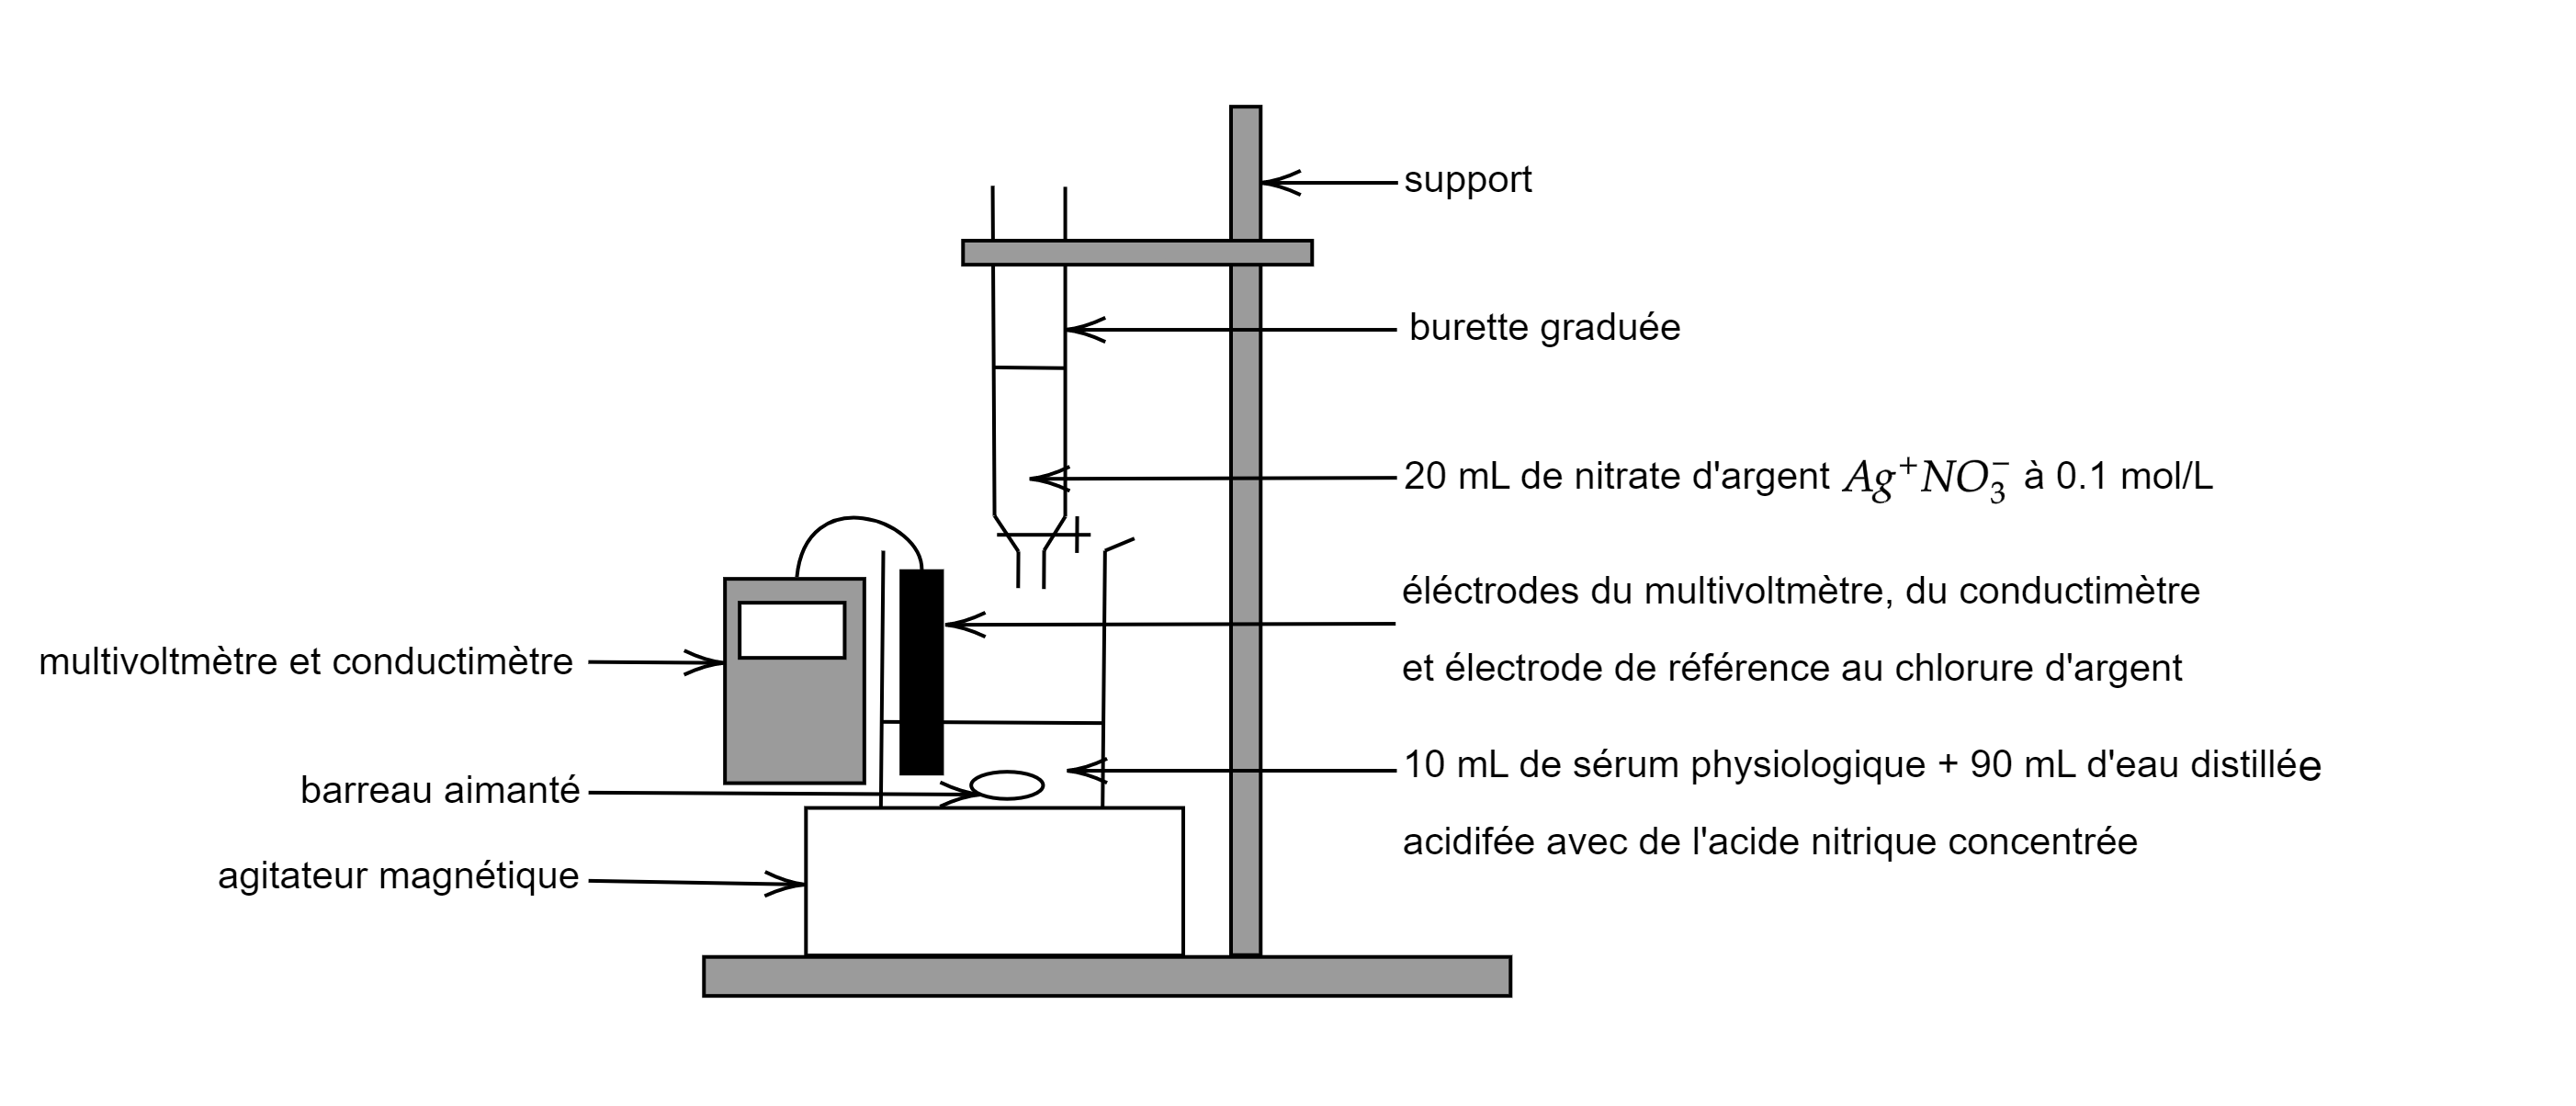
\includegraphics[scale=0.2]{Schema_montage.png}
        \caption{Schéma du montage expérimental du dosage potentiométrique et conductimétrique des ions chlorure par le nitrate d'argent}
        \label{img1:Schema_montage}
    \end{center}
\end{figure}


\section{Observations et résultats}

Dès qu'on commence à verser du nitrate d'argent, un précipité blanc se forme dans le bécher. 
On regroupe nos mesures de potentiel et de conductimétrie sous forme de graphiques.

\begin{figure}[p!]
    \begin{center}
        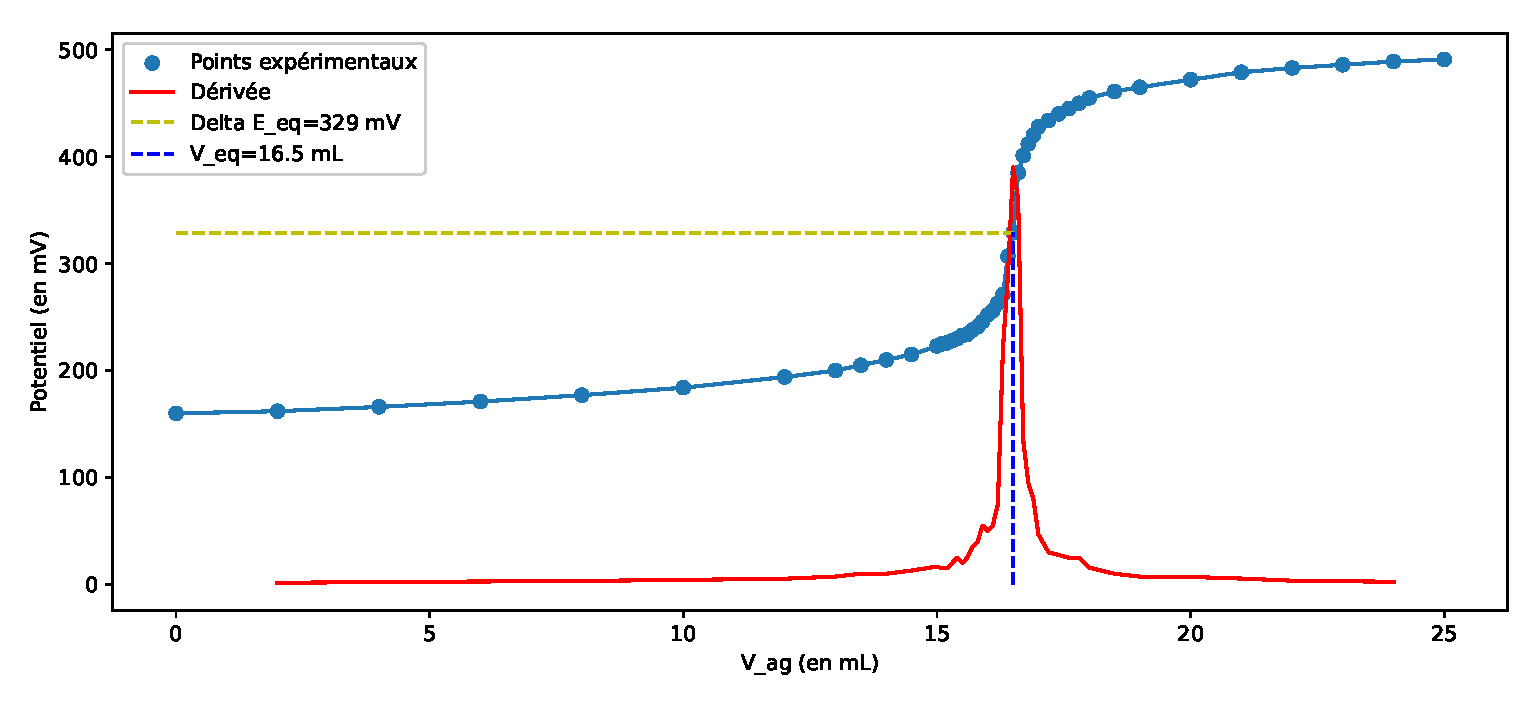
\includegraphics[scale=0.9,angle=90]{Potentiel.eps}
        \caption{Graphiques du potentiel mesuré en fonction du volume d'argent versé. La courbe en rouge correspond à la dérivée en chaque point.}
        \label{img2:Potentiometrie}
    \end{center}
\end{figure}

\begin{figure}[p!]
    \begin{center}
        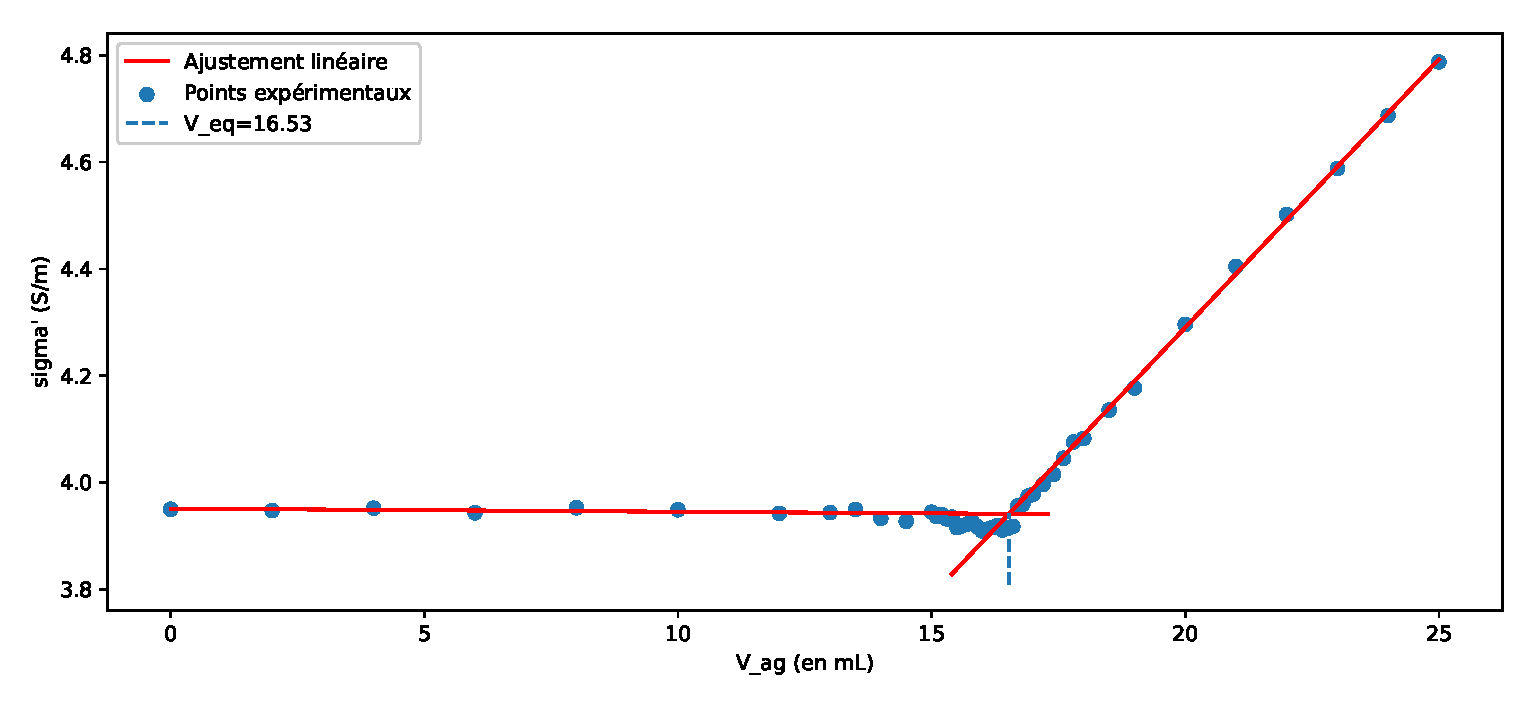
\includegraphics[scale=0.9,angle=90]{Conducti.eps}
        \caption{Graphique de $\sigma '$ en fonction du volume d'argent versé. $\sigma '$ correspond à $\sigma$ la conductance mesurée multipliée par un facteur de dilution $\frac{v_{ag}+v_{t0}}{v_{t0}}$}
        \label{img3:Condu}
    \end{center}
\end{figure}

\newpage
\section{Interprétations}

La réaction de dosage est :
\begin{equation}
    Ag^+_{(aq)} + Cl^-_{(aq)} \longrightarrow AgCl_{(s)}
    \label{eq1:reaction_dosage}
\end{equation}

Le précipité blanc qui se forme pendant le dosage est donc du chlorure d'argent $AgCl$.
On note $v_0=10 \ mL$ le volume initial de sérum physiologique prélevé, $v_{t0}=100 mL$ le volume d'eau et de sérum physiologique dans le bécher avant le dosage.
$v_{ag}$ est le volume d'argent versé et $c_{ag}=0.1 \ M$ la concentration de la solution de nitrate d'argent. 

Le volume équivalent est déterminé de deux manières. 

Par potentiométrie : on utilise la méthode de la dérivée sur le graphique (\ref{img2:Potentiometrie}) et on obtient $v_{eq1}= 16.5 \pm 0.1 \ mL $, l'incertitude sur le volume venant de l'incertitude de la burette graduée.
À l'équivalence, on a d'après la réaction (\ref{eq1:reaction_dosage}):
\begin{align*}
    n_{Ag}=n_{Cl} & \Longrightarrow  v_{eq1} \times c_{ag} = v_{0} \times c_{\phi 1} \\ 
    n_{Ag}=n_{Cl} & \Longrightarrow  c_{\phi 1} = \frac{v_{eq1} \times c_{ag}}{v_{0}} \\
    n_{Ag}=n_{Cl} & \Longrightarrow  c_{\phi 1} = \frac{16.5 \times 0.1}{10} \\
    n_{Ag}=n_{Cl} & \Longrightarrow  c_{\phi 1} = 0.165  \ M
\end{align*}

$c_{\phi 1}$ est la concentration en ions chlorure du sérum physiologique. 
On peut calculer l'incertitude associée :
\begin{align*}
    \Delta c_{\phi 1} & = c_{\phi 1} \times \left(\frac{\Delta v_{eq1}}{v_{eq1}} + \frac{Delta v_0}{v_0} \right) \\
    \Delta c_{\phi 1} & = 0.165 \times \left( \frac{0.1}{16.5} + \frac{0.02}{10} \right) \\
    \Delta c_{\phi 1} & = 0.001 \ M
\end{align*}

On obtient donc $c_{\phi 1}= 0.165 \pm 0.001 \ M$.
On calcule le titre massique du sérum physiologique : $t_{\phi 1}=c_{\phi 1} \times M_{NaCl}=0.165 \times 58.44 = 9.64 \ g.L^{-1}$.
On calcule facilement l'incertitude associée et on obtient $t_{\phi 1}=9.64 \pm 0.06 \ g.L^{-1}$.

On calcule le pKs du chlorure d'argent. On utilise la relation de Nerst : 
\begin{align*}
    E(Ag^+/AgCl)& = E^0(Ag^+/AgCl) + \frac{R T}{F}ln(\frac{a_{Ag^+}}{a_{AgCl}}) \\
    E(Ag^+/AgCl)& = E^0(Ag^+/AgCl) + \frac{R T}{F}ln(10) log([Ag^+])
\end{align*}

À l'équivalence on a $[Ag^+]= \sqrt{pKs}$, et si on note $\Delta E$ le potentiel mesuré par rapport à l'électrode de référence au chlorure d'argent on obtient :
\begin{equation}
    \Delta E = E(Ag^+/AgCl) - E_{ref} \Longrightarrow pKs = \frac{2 \times F}{R \times F \times ln(10)}(E^0(Ag^+/AgCl)-\Delta E - E_{ref})
    \label{eq2:pKs}
\end{equation}

On mesure une température dans la pièce $T=20^\circ C$ et avec le graphique (\ref{img2:Potentiometrie}) on a $\Delta E = 0.329 V $.
En utilisant ces valeurs et $E^0(Ag^+/AgCl)=0.8 \ V/ESH$,$E_{ref}= 0.197 \ V/ESH$ dans l'équation (\ref{eq2:pKs}):
\begin{align*}
    pKs &= \frac{2 \times 96500}{8.314 \times ln(10) \times 293.15}(0.8-0.329-0.197) \\
    pKs &= 9.42
\end{align*}

On a donc pKs=9.42.

Par conductimétrie : On trace $\sigma ' =\sigma \times \frac{v_{ag}+v_{t0}}{v_{t0}}$ et on fait une régression linéaire pour les points avants et les points après l'équivalence.
On calcule le point d'intersection de ces deux droites et l'abscisse nous donne le volume équivalent.
On obtient sur le graphique (\ref{img3:Condu}) $v_{eq2}=16.53 \ mL$. 

On calcule la concentration :
\begin{align*}
    c_{\phi 2} &= \frac{v_{eq2}\times c_{Ag}}{v_0} \\
    c_{\phi 2} &= 0.1653 \ M
\end{align*}

On obtient $ c_{\phi 2} = 0.1653 \ M $. On calcule le titre massique $t_{\phi 2}=9.66 \ g.L^{-1}$.

\section*{Conclusion}

Dans ce travail pratique nous avons dosé par conductimétrie et potentiométrie les ions chlorures d'un sérum physiologique par du nitrate d'argent.

Nous avons obtenu pour le chlorure d'argent $pKs_{exp}=9.42$ la valeur théorique est $pKs_{theo}=9.752$. 
On a un écart relatif de $\frac{9.752-9.42}{9.752}= 4 \%$. 
Cet écart peut-être expliqué par l'incertitude sur le potientiel que nous n'avons pas pris en compte et sur la différence de température.
Une constante de réaction dépend de la température. 
Nous avons calculé le pKs pour $20^\circ C$ mais le valeur théorique utilise sûrement une température de $25^\circ C$.

Nous avons obtenue des titres massiques $t_{\phi 1}= 9.64 \pm 0.06 \ g.L^{-1}$ pour la potentiométrie et $t_{\phi 1}= 9.66 \ g.L^{-1}$.
Ces deux valeurs sont cohérentes entre elles. 
La valeur théorique est $t_{\phi \ theo}= 9.0 \ g.L^{-1}$.
On trouve pour les deux méthodes un écart relatif de $7\ \%$.
Cet écart est significatif et n'est pas expliqué par nos incertitudes.
D'autres groupes qui ont réalisé ce travail pratique trouve un écart significatif avec la valeur théorique, notre résultat est donc reproductible.
On conclut que le titre massique théorique est faux. 


\end{document}